\chapter{KERANGKA KONSEPTUAL PENELITIAN}

\section{Permasalahan dan Tantangan Penelitian}

Dalam pengertian yang sangat luas, orang biasa mengenal data mining dengan pengolahan data dengan berbagai macam teknik dengan ukuran data yang beragam. Data \textit{mining} sebagai bidang yang menggabungkan bidang‐bidang keilmuan terkait seperti pengenalan pola, \textit{database}, \textit{machine learning}, statistik, serta  visualisasi guna menangani masalah-masalah dalam mengambil suatu informasi dari banyaknya data yang ada. Data mining merupakan suatu proses yang memanfaatkan \textit{artificial intelligence}, teknik statistik, \textit{machine learning}, dan juga matematika guna melakukan identifikasi dan ekstraksi informasi serta suatu pengetahuan yang sekiranya akan bermanfaat dari berbagai database yang berukuran besar (Decision Support Systems and Intelligent Systems 7th Edition (PDFDrive).Turban, 2015)

\textit{Clustering} adalah salah satu metode data mining dimana sekelompok data akan dibagi ke dalam beberapa kelompok yang terbentuk secara alami berdasarkan  kesamaan karakteristik  data  masing-masing  dalam sebuah  dataset yang besar \citep{Singh2011}. Terkait dengan penelitian ini, terdapat penelitian‐penelitian     yang telah  dilakukan  sebelumnya, baik tentang media pembelajaran digital maupun tentang algoritma yang digunakan, yakni \textit{Self‐Organizing Map} (SOM) dan juga kombinasinya dengan m-aT. Penelitian-penelitian terdahulu ini digunakan sebagai landasan dalam proses penelitian.

Pada tahun 2019, sebuah penelitian tentang memetakan siswa berdasarkan aktivitasnya di media pembelajaran digital pernah dilakukan secara manual. Dalam penelitian ini, analisis dilakukan secara manual dengan mengambil kesimpulan melalui visualisasi dan persepsi peneliti. Siswa dipetakan menjadi empat kelompok berdasarkan pola siswa dalam menyelesaikan permasalahan dalam Monsakun. Hasil pemetaan dapat mengatakan bahwa siswa disetiap kelompok membutuhkan perlakuan yang berbeda-beda \citep{SupiantoHayashiHirashima2019}.

Sebuah penelitian dengan adaptasi lebih lanjut dari pemetaan performa belajar siswa juga telah dilakukan. Penelitian ini dilakukan untuk mengelompokan siswa pengguna \textit{E-Learning} secara otomatis dengan menggunakan algoritme SOM. Data yang digunakan dalam penelitian ini merupakan sekumpulan data interaksi dan aktivitas siswa yang mengambil mata pelajaran  Algoritme dan  Struktur Data ketika  menggunakan \textit{E‐Learning}. Pada penelitian ini, atribut yang digunakan dipilih menggunakan \textit{Principal Component Analysis} (PCA) terlebih dahulu sebelum kemudian diproses dengan SOM. Kemudian melalui proses tersebut, dihasilkan \textit{Low Browsing cluster} dan \textit{High Browsing cluster}. Adapun pengujian yang dilakukan dalam penelitian ini dengan menggunakan \textit{Silhouette index}, \textit{Dunn index}, dan \textit{Davies-Bouldin index} dan membandingkannya dengan K-Means dan \textit{Partitioning Around Medoids} dan memunculkan SOM sebagai algoritma yang cukup baik untuk melakukan \textit{Clustering} terhadap log data aktivitas siswa karena memiliki hasil terbaik pada nilai Silhouette index sebesar $0.4502$ dan \textit{Dunn index} sebesar $1.1452$ \citep{Alias2017}.

Selain digunakan dalam bidang pendidikan, SOM juga banyak digunakan dalam  bidang-bidang  lainnya. Salah  satunya  adalah  penelitian  yang  dilakukan oleh Dini dan \citet{Dini2020}, bahwa hasil \textit{Clustering} 34 provinsi di Indonesia dengan indikator kesejahteraan masyarakat yang terdiri dari enam indikator diperoleh metode terbaik dengan menggunakan analisis \textit{cluster K-Means}. Analisis \textit{cluster K-Means} dipilih karena didasarkan pada nilai varians $(0,101)$ yang lebih kecil dari nilai varians Average Linkage Clustering $(0,152)$. Selain itu, diketahui bahwa kesejahteraan masyarakat di Indonesia Indonesia masih belum merata. Hal ini dapat dilihat pada karakteristik masing-masing \textit{cluster}. Setiap kelompok memiliki prioritas yang berbeda dalam yang berbeda dalam bidang kesejahteraan yang perlu diperhatikan atau ditingkatkan oleh pihak-pihak terkait. Provinsi-provinsi yang berada di kelompok pertama dapat menjadi prioritas dalam berbagai aspek kesejahteraan bagi pemerintah agar kesejahteraan dapat dirasakan secara adil oleh masyarakat. Kesejahteraan dapat dirasakan secara adil oleh masyarakat. Sementara itu, provinsi yang berada di kelompok kedua dan ketiga masih perlu mendapat perhatian dalam beberapa aspek kesejahteraan masyarakat. Visualisasi kelompok dalam bentuk peta Indonesia diharapkan dapat memudahkan untuk menggambarkan kondisi umum kesejahteraan provinsi-provinsi di Indonesia \citep{Dini2020}.

Tak hanya itu, SOM juga digunakan pada penelitian lain di berbagai bidang sesuai  keahlian  masing-masing  peneliti.  Seperti  penelitian  yang  dilakukan  oleh \citet{Oliver2018} di bidang biologi, atau penelitian yang dilakukan oleh \citet{Pisano2017} dan \citet{MolinaGarcia2019} di bidang kesehatan. Penelitian-penelitian  ini membuktikan bahwa algoritme SOM tidak hanya dapat digunakan untuk bidang tertentu seperti pendidikan saja, melainkan dapat digunakan pula untuk bidang-bidang lainnya.
Penelitian  lain  yang  juga  menjadi  acuan  penelitian  ini  adalah  penelitian-penelitian yang menggunakan pengembangan dari algoritme SOM konvensional dalam prosesnya. Salah satunya adalah penelitian yang bergerak di bidang Biologi dengan menggunakan dua jenis dataset, yakni \textit{Human Fibroblasts Serum} (HFS) dataset dan Rat CNS dataset. Kedua data kemudian diolah dan divisualisasikan dengan menggunakan algoritme SOM. Map size yang dihasilkan pada HFS cukup beragam, yakni $6×2$, $4×3$, dan $3×4$. Sementara CNS mengeluarkan ukuran yang sama, yakni 3×3. Setelah data selesai diolah, data diuji dengan menggunakan Silhouette index. Hasil pengujian dalam penelitian ini menunjukkan nilai \textit{Silhouette} sebesar lebih dari 0.6 untuk setiap data HFS, dan $0.5927942$ untuk seluruh data CNS. Selanjutnya algoritme SOM yang telah dikembangkan dalam penelitian ini disebut dengan SOMHS \citep{George2015}. 

Mayoritas pengembangan dari SOM konvensional hanya bisa digunakan pada kasus tertentu saja. Namun, sebuah penelitian lain yang juga merupakan pengembangan dari SOM berhasil dilakukan pada tahun 2019. Penelitian ini membahas mengenai kombinasi dari penggunaan \textit{Self Organizing Map} (SOM) dan \textit{Fuzzy C-Means} (FCM) dalam \textit{Clustering} yang bertujuan untuk mengevaluasi kualitas air tanah di Seoul, Korea Selatan. Penelitian tersebut  mengatakan bahwa SOM dan FCM yang sama-sama mampu diterapkan dalam sekumpulan data besar yang kompleks akan saling melengkapi jika dikombinasikan. Hal ini terjadi karena baik SOM dan FCM sama-sama memiliki kekurangan dan saling membutuhkan. SOM yang dikenal dengan visualisasinya seringkali memunculkan ambiguitas pada keluarannya hingga FCM dirasa  cocok untuk  membantu  menciptakan batasan-batasan  kelompok  dari  hasil keluaran SOM tersebut. Kedua algoritme ini juga mudah diterapkan sehingga dapat  diimplementasikan tidak hanya pada kasus-kasus  tertentu \citep{Lee2019}.

Penambangan atau eksplorasi data adalah bagian dari area penelitian terbaru  yang lebih luas dalam Kecerdasan Buatan dan Pemrosesan dan Manajemen Informasi atau dikenal sebagai \textit{Knowledge Discovery in Database} (KDD). Tujuannya untuk mengidentifikasi informasi atau pengetahuan baru dari database di mana dimensi atau jumlah data sangat besar sehingga melampaui pemahaman manusia. MST digunakan untuk menganalisis basis data transformator daya dari satu dari penyedia energi listrik di Jepang. Evaluasi kelompok dihasilkan oleh SOM biasanya dilakukan oleh mata manusia. Karena sifatnya kualitatif alam, evaluator dapat melebih-lebihkan atau meremehkan jumlah kelompok yang terbentuk di peta. Dengan pendekatan ini, tepat jumlah kelompok yang dihasilkan oleh peta tidak dapat dikonfirmasi karena salah tafsir dari ekspresi tingkat abu-abu (Tokutaka et al., 2001).
Penelitian tentang teknik visualisasi menggunakan SOM dan MST. Metode ini dapat mengungkapkan kelompok barang serupa, berdasarkan graf yang dibangun baik dari data input, atau node SOM. Evaluasi visualisasi, dan membandingkannya dengan metode graf kerapatan, dan menemukannya untuk mengungkapkan informasi serupa. Visualisasi tidak bergantung pada parameter pengguna tertentu, yang bermanfaat bagi pengguna pemula. Metode operasi pada simpul SOM umumnya memiliki waktu komputasi yang lebih rendah daripada metode graf kepadatan, karena jumlah node dalam SOM umumnya besarnya lebih kecil dari jumlah sampel data \citep{MayerRauber2010}.

Penelitian algoritma SOM-MST yang menggabungkan SOM dengan graf MST dan membahas bagaimana MST dari sebuah graf yang mencapai subset sisi yang paling ekonomis yang menghubungkan semua komponen dengan sebuah \textit{loop} terbuka. Dalam penelitian ini, MST pada SOM dengan sub-simpul yang disematkan dan ukuran jarak untuk pilihan ukuran dan bentuk peta yang optimal. Penelitian ini mendemonstrasikan dengan menggunakan data \textit{Fisher's Iris} dan data ekspresi gen yang nyata. Kumpulan data simulasi juga dianalisis untuk memeriksa validitas metode yang diusulkan (Jang et al., 2009).

Penelitian yang terkait dengan kombinasi SOM dan teori graf adalah SOM graf teoretis ke domain data hierarkis. Hasilnya memiliki kompleksitas algoritmik yang lebih rendah daripada SOM asli,dan dapat menghasilkan SOM yang memiliki validitas kelompok yang jauh lebih tinggi daripada pengkodean biner \citep{Argyrou2009}, menggunakan pemetaan probabilitas selama \textit{Graph}-SOM \citep{Hagenbuchner2009}, pelatihan \textit{Graph}-MST-SOM membantu meningkatkan kinerjanya secara signifikan dan membantu secara substansial mengurangi permintaan komputasi \citep{MayerRauber2010,Resta2016} dan hasilnya mendukung penggunaan pendekatan teoretis graf seperti dalam semua eksperimen jumlah kelompok yang ditemukan sudah benar dan valid \citep{Silva2011}.

Heba Mohmmed Nagy Rashad, 2013, meneliti tentang Penambangan data pendidikan adalah bidang penambangan data tertentu diterapkan pada data yang berasal dari lingkungan pendidikan, bergantung pada pendekatan yang berbeda untuk menemukan pengetahuan yang tersembunyi dari data yang tersedia. Di antara pendekatan tersebut adalah teknik pembelajaran mesin yang digunakan untuk membangun sistem yang memperoleh pengetahuan tersembunyi dari data sebelumnya. Pembelajaran mesin dapat diterapkan untuk memecahkan masalah yang berbeda regresi, klasifikasi, \textit{Clustering} dan optimasi masalah. 

Dalam penelitian ini mengusulkan “Penasehat Siswa” yang adapun permasalahan dan tantangan dalam penelitian ini untuk menerapkan kombinasi dari algoritme SOM dan m-aT di bidang penambangan data Monsakun sebagai data pendidikan. Data yang digunakan dalam penelitian ini merupakan log data yang dihasilkan melalui rekaman aktivitas belajar belajar siswa pada media pembelajaran digital bernama Monsakun. Selanjutnya melalui sebuah proses pengolahan, data tersebut akan menghasilkan \textit{Clustering} siswa dan sistem penasehat guru yang dapat digunakan untuk \textit{Clustering} performa belajar siswa agar umpan balik siswa ke guru atau sebaliknya yang tepat dapat diberikan sebagai dasar melakukan evaluasi pembelajaran problem posing integrasi kalimat  cerita aritmatika.

\section{Ide Umum Penelitian}
Ide umum penelitian ini adalah:
\begin{enumerate}
	\item Untuk membuat analisis proses \textit{Clustering} siswa.
	\item Untuk penasehat pembelajaran oleh guru dalam problem posing melalui integrasi kalimat Cerita Aritmatika menggunakan \textit{Self-Organizing Map-m-Ary Tree} (SOM-m-aT).
	\item Persepsi guru Sekolah Dasar di Indonesia tentang sistem penasehat pembelajaran berdasarkan kemiripan siswa.
\end{enumerate}

\begin{figure}[h]
	\centering
	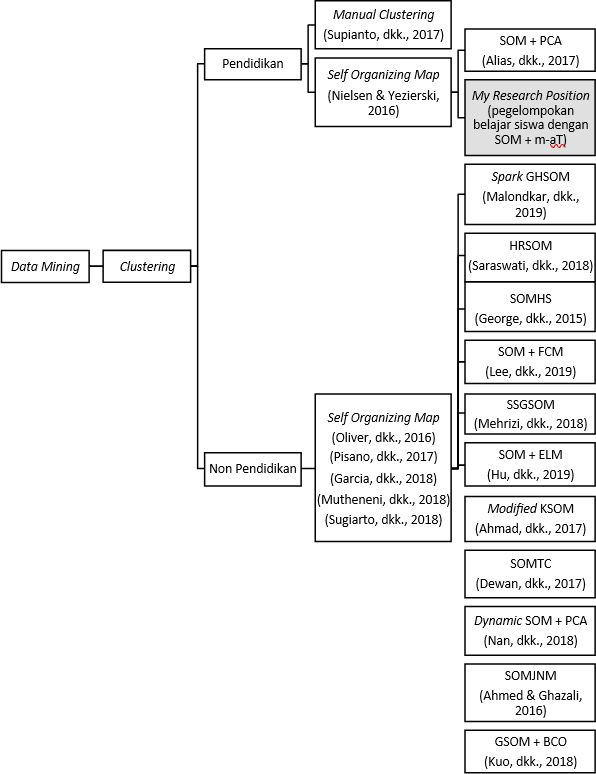
\includegraphics[width=0.5\textwidth]{Gambar/bagankerangka}
	\caption{Bagan kerangka konseptual penelitian}
	\label{fig:g5}
\end{figure}

\begin{landscape}
	\begin{center}
		\renewcommand{\arraystretch}{1.2}
		\setlength\extrarowheight{2pt}
		
		\begin{tabularx}{\linewidth}{|Y|Y|c|Y|Y|Y|}
			\caption{Matriks pemetaan posisi penelitian untuk metode penelitian dengan SOM dan Graf} \label{tab:1} \\
		
			\hline
			\textbf{Nama Peneliti} & \textbf{Judul Paper} & \textbf{SOM} & \textbf{Graf} & \textbf{Dataset} & \textbf{Jenis Paper} \\
			\hline
			\endfirsthead
			
			\hline
			\textbf{Nama Peneliti} & \textbf{Judul Paper} & \textbf{SOM} & \textbf{Graf} & \textbf{Dataset} & \textbf{Jenis Paper} \\
			\hline
			\endhead
			
			Argyris Argyrou, 2009 & \textit{Clustering Hierarchical Data Using Self-Organizing Map: A Graph-Theoretical Approach}
			& $\checkmark$ & teori graf & the zoo-dataset [9] berisi 101 binatang & Prosiding \\ \hline
			
			Markus Hagenbuchner, dkk., 2009 & \textit{Projection of undirected and non-positional graphs using Self Organizing Maps}
			& - & \textit{Probabilitas mapping Graph SOM (PM-Graph-SOM).} & Terdiri dari 114, 366 yang melalui hyperlinks. & Prosiding \\ \hline
			
			Rudolf Mayer dan Andreas Rauber, 2010 & \textit{Visualising Clusters in Self-Organising Maps with Minimum Spanning Trees}
			& - & MST & Iris & Prosiding \\ \hline
			
			Leandro A. Silva dan José Alfredo F. Costa, 2011 & \textit{A Graph Partitioning Approach to SOM Clustering}
			& - & \textit{Graph Partitioning Approach} & \textit{Synthetic, Spiral, Iris-database} & Prosiding \\ \hline
			
			Marina Resta, 2012 & \textit{Graph Mining Based SOM: A Tool to Analyze Economic Stability}
			& - & MST & Ekonomi & Book Chapter \\ \hline
			
			Marina Resta, 2015 & \textit{Enhancing Self-Organizing Map Capabilities with Graph Clustering : An Application to Financial Markets}
			& - & MST & Keuangan & Prosiding \\ \hline
			
			Supianto, A.A., dkk., 2016 & \textit{Visualizations of problem-posing activity sequences toward modeling the thinking process.}
			& - & - & $\checkmark$ Monsakun Data & Jurnal \\ \hline
			
			Supianto, A.A., dkk., 2017 & \textit{Model-based analysis of thinking in problem posing a sentence integration focused on violation of the constraints}
			& - & - & $\checkmark$ Monsakun Data & Jurnal \\ \hline
			
			Puteri Nor Ellyza Nohuddin, dkk., 2018 & \textit{Monitoring Students Performance using Self Organizing Map Trend Clustering}
			& - & - & - & Jurnal \\ \hline
			
			Musa Wakil Bara, dkk., 2018 & \textit{Self-Organizing Map Clustering Method for the Analysis of E-Learning Activities}
			& - & - & UTM Moodle LMS log records. & Prosiding \\ \hline
			
			Abla Chaouni Benabdellah, dkk., 2019 & \textit{A survey of clustering algorithms for an industrial context}
			& - & - & Logistik, kebutuhan Pelanggan, Sistem kualitas Otomotif dan Pesawat & Prosiding \\ \hline
			
			Fitri Latifah, 2016 & \textit{Penerapan Algorithma Pohon untuk Operasi Pengolahan dan Penyimpanan Data dalam Teknik Pemrograman}
			& - & $\checkmark$ \textit{m-ary-tree} & Data Teknik Pemrograman & Jurnal \\ \hline
			
			César A. Astudillo dan B. John Oommen, 2009 & \textit{On Using Adaptive Binary Search Trees to Enhance Self Organizing Maps}
			& - & Graf pohon (BST) & TTO-CONROT dataset & Prosiding \\ \hline
			
			Nabila Divanadia Luckyana, dkk., 2021 & \textit{Implementasi Kombinasi Algoritme Self-Organizing Map dan Fuzzy C-Means untuk Clustering Performa Belajar Siswa pada Media Pembelajaran Digital}
			& - & - & $\checkmark$ Data Monsakun & Prosiding \\ \hline
			
			Tibyani, dkk, 2022 & - & - & $\checkmark$ \textit{m-ary-tree} & $\checkmark$ Data Monsakun & Jurnal dan Prosiding \\ \hline
			
		\end{tabularx}
	\end{center}
\end{landscape}


\begin{landscape}
	\begin{table}
		\centering
		\renewcommand{\arraystretch}{1.2}
		\setlength\extrarowheight{2pt}
		\caption{Matriks pemetaan posisi penelitian untuk metode penelitian sistem penasehat oleh guru atau dosen}
		\label{tab:2}
		\begin{tabularx}{\linewidth}{|Y|Y|c|Y|c|}
			\hline
			\textbf{Nama Peneliti} & \textbf{Judul} & \textbf{Teknologi} & \textbf{Dataset} & \textbf{Jenis Paper} \\
			\hline
			Heba Mohmmed Nagy Rashad, 2013 & \textit{Automated Student Advisory using Machine Learning} & Web & Institut Tinggi Kairo untuk Teknik, Ilmu Komputer, dan Manajemen menggunakan data yang dikumpulkan selama 12 tahun (2000–2012) & Jurnal \\
			\hline
			Olawande Daramola, dkk., 2014 & \textit{Implementation of an Intelligent Course Advisory Expert System} & $\checkmark$ & Dari Department of Computer and Information Sciences of Covenant University Nigeria & Jurnal \\
			\hline
			Ikono Rhoda Nsikan-Abasi, dkk., 2016 & \textit{Engineering of a Student Advisory Management System: Development Perspective} & $\checkmark$ & 24 Penasehat dari tujuh (7) fakultas Universitas Obafemi Awolowo, Nigeria. 120 siswa dipilih secara acak dari masing-masing fakultas & Jurnal \\
			\hline
			Tawafak, R.M., dkk., 2020 & \textit{A Review Paper on Student-Graduate Advisory Expert System} & – & Databases \textit{IEEE, Scopus, ScienceDirect, E-database}, dan \textit{ResearchGate} dengan total artikel 107,932 & Prosiding \\
			\hline
			Bamo Nadir Faraj dan Aree Ali Muhammed, 2021 & Online Course Registration and Advisory Systems Based on Students’ Personal and Social Constraints & $\checkmark$ & Data dari Komar University of Science and Technology (KUST), Irak & Jurnal \\
			\hline
		\end{tabularx}
	\end{table}
\end{landscape}
